%
% problem.tex -- Problemstellung
%
% (c) 2021 Prof Dr Andreas Müller, OST Ostschweizer Fachhochschule
%
\bgroup
\begin{frame}[t]
\setlength{\abovedisplayskip}{5pt}
\setlength{\belowdisplayskip}{5pt}
\frametitle{Brachistochrone}
\vspace{-10pt}
\begin{center}
\pgfmathparse{12/(2*3.1415)}
\xdef\r{\pgfmathresult}
\begin{tikzpicture}[>=latex,thick]
\uncover<1-2>{
\node at (6,-1.8) {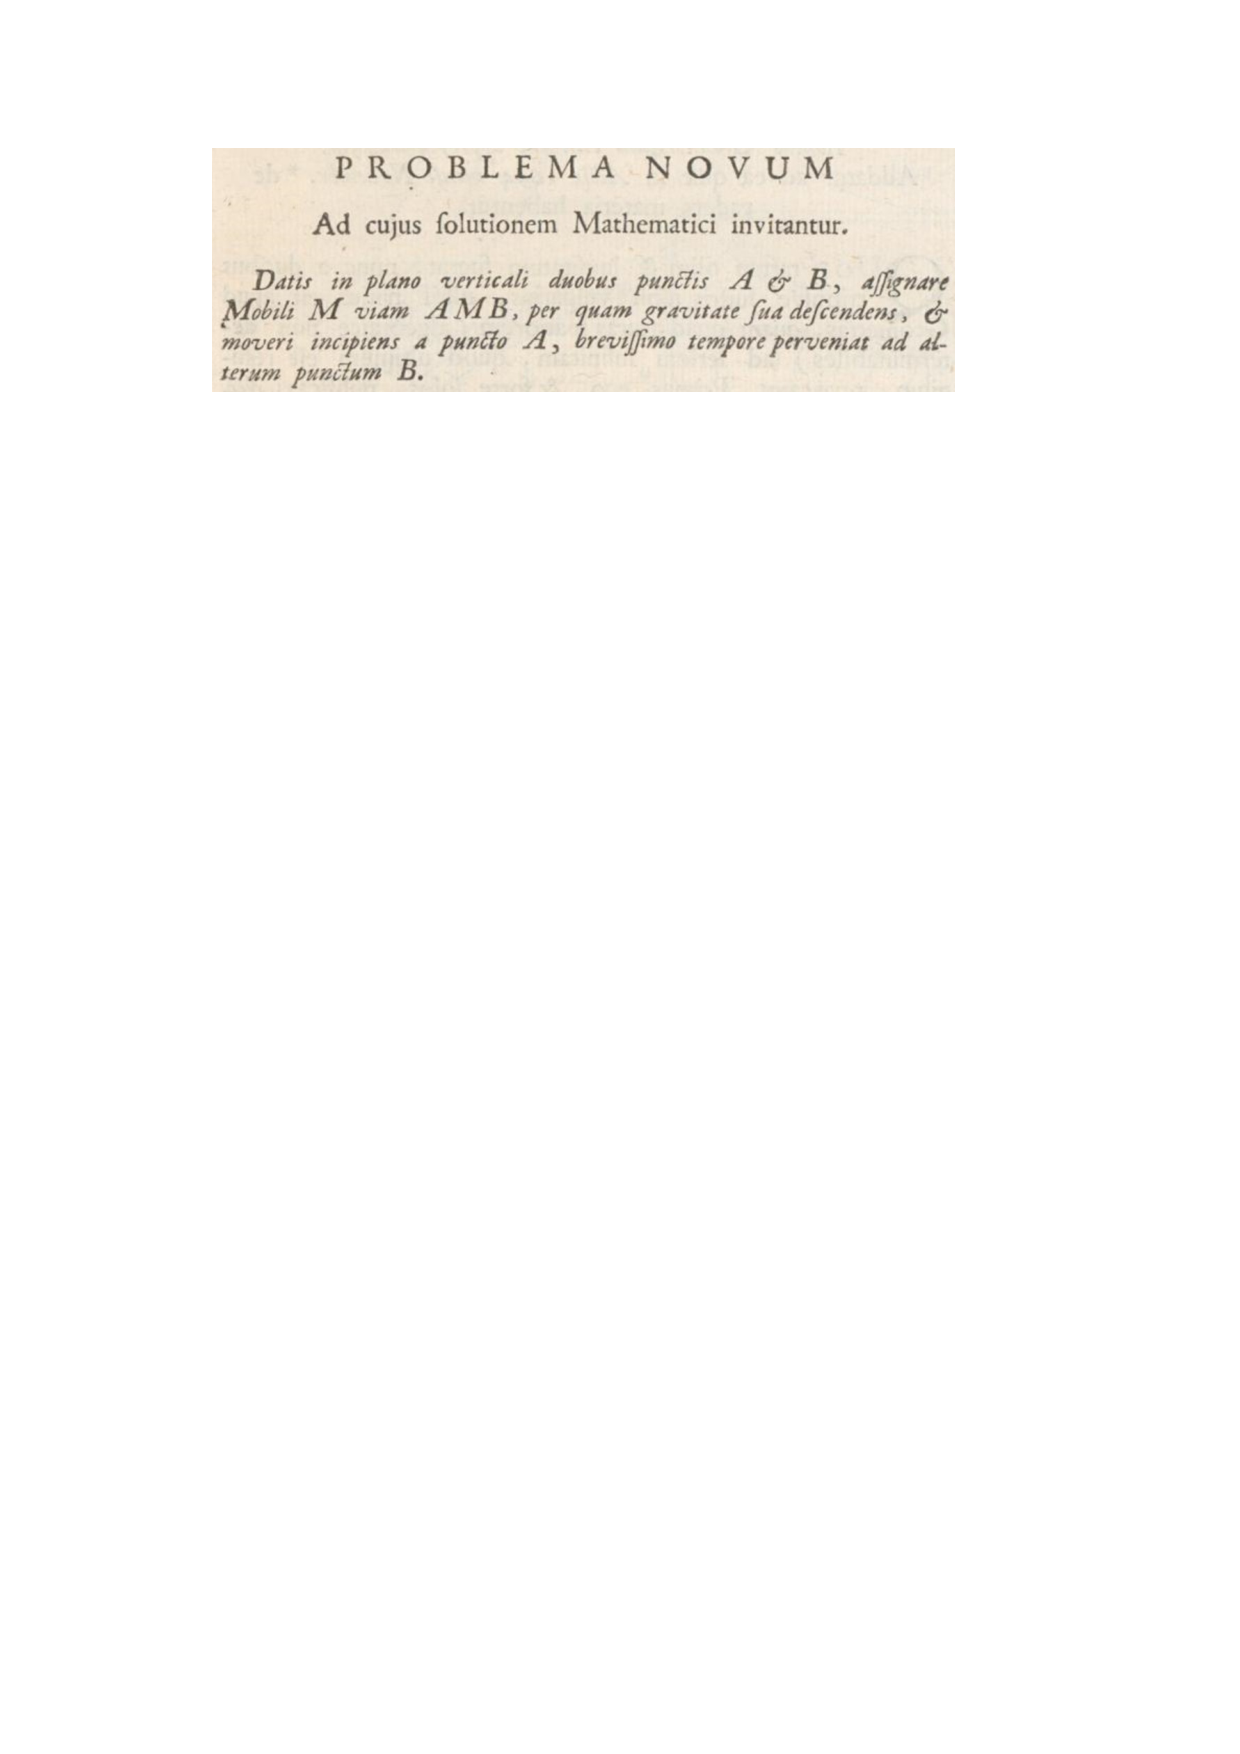
\includegraphics[width=13cm]{../slides/0/latein.pdf}};
}
\uncover<6->{
	\draw[color=red!50!black,line width=1.2pt]
		plot[domain=0:360,samples=100]
			({\r*3.1415*\x/180-\r*sin(\x)},{\r*(cos(\x)-1)});
}
\uncover<5->{
	\draw[color=red,line width=2pt]
		plot[domain=40:170,samples=100]
			({\r*3.1415*\x/180-\r*sin(\x)},{\r*(cos(\x)-1)});
}
\uncover<3->{
	\def\x{40}
	\fill[color=red]
		({\r*3.1415*\x/180-\r*sin(\x)},{\r*(cos(\x)-1)})
			circle[radius=0.1];
	\node at 
		({\r*3.1415*\x/180-\r*sin(\x)},{\r*(cos(\x)-1)})
			[right] {$A$};
	\def\x{170}
	\fill[color=red]
		({\r*3.1415*\x/180-\r*sin(\x)},{\r*(cos(\x)-1)})
			circle[radius=0.1];
	\node at 
		({\r*3.1415*\x/180-\r*sin(\x)},{\r*(cos(\x)-1)})
			[above] {$B$};
}
\uncover<4->{
	\def\x{100}
	\fill[color=red]
		({\r*3.1415*\x/180-\r*sin(\x)},{\r*(cos(\x)-1)})
			circle[radius=0.1];
	\node at 
		({\r*3.1415*\x/180-\r*sin(\x)},{\r*(cos(\x)-1)})
			[above right] {$M$};
}
\uncover<6->{
	\draw[->] (-0.5,0) -- (12.5,0) coordinate[label={$x$}];
	\draw[->] (0,0.5) -- (0,-4) coordinate[label={right:$y$}];
}
\end{tikzpicture}
\end{center}
\uncover<2->{%
\begin{quote}
Neue Aufgabe, zu deren Lösung die Mathematiker eingeladen werden.
Gegeben zwei Punkte $A$ und $B$ in einer vertikalen Ebene, finde
die Bahn $AMB$ eines Punktes $M$, der unter der Wirkung seines Gewichtes
in kürzester Zeit vom Punkt $A$ zum anderen Punkt $B$ absteigt.
\end{quote}}
\end{frame}
\egroup
